\chapter{Implementatie}

\section{Technologi\"en}

Wij hebben gekozen voor de volgende technologi\"en voor het ontwikkelen van deze webapplicatie:
\begin{itemize}
	\item Groovy - Een dynamische en behendig object geori\"enterd taal gebaseerd op de taal Java.
	\vspace{2mm} \\
	\textit{Wij hebben hiervoor gekozen omdat Java niet de meest prettig taal is om mee te ontwikkelen maar de Java Virtual Machine, waar Groovy ook op draait, heel stabiel en veilig is. Groovy is maakt gebruikt van de sterkt punten van Java en verbetert de tekorkommingen.}

	\item Grails - Een webframework voor Groovy met de motto ``Convention over configuration''. Het is gefocused op het snel en makkelijk opzetten van webapplicaties.
	\vspace{2mm} \\
	\textit{Wij hebben hiervoor gekozen omdat dit het best ontwikkeld en langst bestand webframework is voor Groovy. Hun ontwikkelings filosofie maakte het ons ook makkelijk om een werkend webapplicatie te maken binnen beperkt tijd.}

	\item Vaadin - Een framework om moderne graphical user interfaces voor webapplicaties te bouwen.
	\vspace{2mm} \\
	\textit{Wij hebben hiervoor gekozen omdat Vaadin het makkelijk maakt om interfaces te maken en tegelijke tijd alle controle over te houden.}
\end{itemize}

\section{Componenten}

\subsection{Checkin}

Als de gebruiker het lab binnen loopt, moet hij eerst inchecken. Om dat mogelijk te maken is een apart pagina gemaakt. Deze pagina is in 
Figuur \ref{fig:checkinoutview} te zien. Het bestaat uit 3 hoofdcomponenten: het welkomsbericht, de checkin knoppen en de checkout tabel.

\begin{figure}[here]
	\centering
	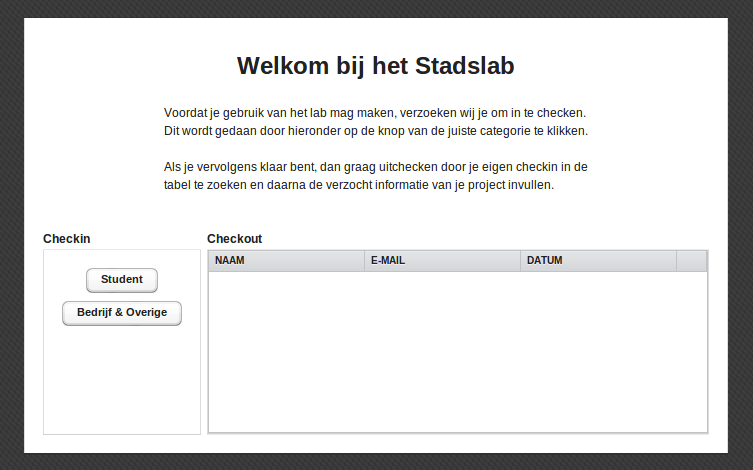
\includegraphics[width=\textwidth]{Images/checkinoutview2.png}
	\caption{Venster waar kan worden ingecheckt en uitgecheckt}
	\label{fig:checkinoutview}
\end{figure}

Het welkomsbericht bestaat uit een korte stuk tekst waarin uitgelegd wordt wat de bedoeling van deze pagina is. \\
Daaronder staan de checkin knoppen. Gebruikers horen de knop te kiezen dat bij hun past, als student of bedrijf/overige zijnde.\\ 
\\
Als een student in wilt checken, dan krijgt de student een venster te zien als weergegeven in Figuur \ref{fig:checkin-student}. Hierbij wordt persoonlijk informatie van de student gevraagd dat door de beheerders gebruikt wordt om bijvoorbeeld kosten te declareren bij de corresponderende instituut. Er wordt verder ook gevraagd met welke apparaten de student zal gaan werken. Hierdoor kunnen de beheerders een overzicht krijgen over welke apparaten de populairste zijn. Verder is er validatie ingebouwd om te zorgen dat alle velden ingevuld zijn, als afgebeeld in Figuur \ref{fig:checkin-student-error}. \\

\begin{figure}[ht]
	\centering
	\subfigure[Checkin met ingevuld gegevens]{
		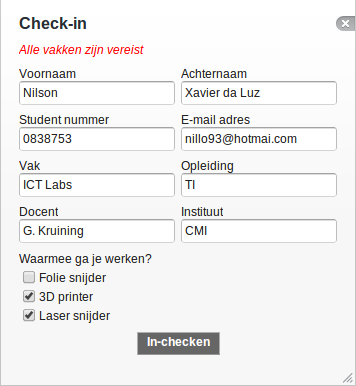
\includegraphics[width=175px, height=225px]{Images/checkin-student.png}
		\label{fig:checkin-student}
	}
	\subfigure[Checkin met errors]{
		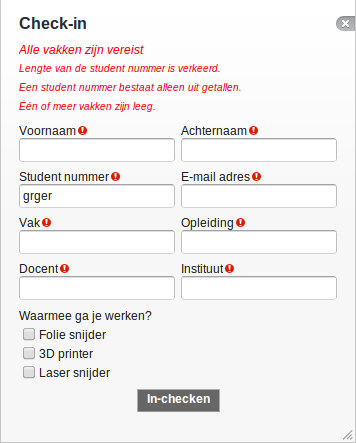
\includegraphics[width=175px, height=225px]{Images/checkin-student-error.png}
		\label{fig:checkin-student-error}
	}
	\caption{Checkin voor studenten}
\end{figure}

Als een bedrijf of overige iemand in wilt checken dat krijgt diegene ook een eigen venster te zien. Hier wordt andere soort informatie gevraagd dat meer bij deze categorie past. Dit venster is te zien bij Figuur \ref{fig:checkin-company}. Ook hier wordt de ingevuld informatie gevalideerd om te zorgen dat alle informatie ingevuld is, dit is weergegeven in Figuur \ref{fig:checkin-company-error}. \\

\begin{figure}[ht]
	\centering
	\subfigure[Checkin met ingevuld gegevens]{
		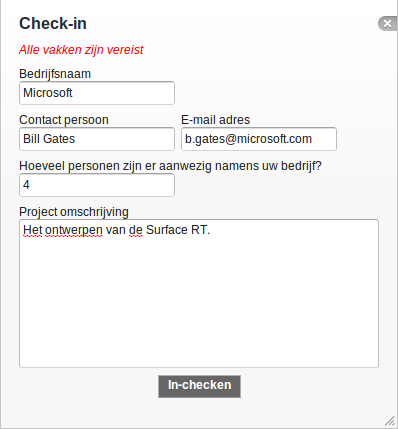
\includegraphics[width=175px, height=225px]{Images/checkin-company.png}
		\label{fig:checkin-company}
	}
	\subfigure[Checkin met errors]{
		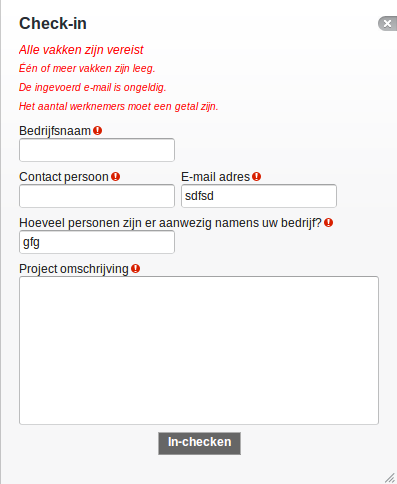
\includegraphics[width=175px, height=225px]{Images/checkin-company-error.png}
		\label{fig:checkin-company-error}
	}
	\caption{Checkin voor bedrijven}
\end{figure}

Zodra de gebruiker heeft ingecheckt, dan is de gebruiker vrij om gebruik te maken van het lab. Er komt dan een nieuwe element in de checkouts tabel te staan met de informatie van de gebruiker en een knop om uit te checken. Dit is te zien in Figuur \ref{fig:checkout-table}. \\

\begin{figure}[ht]
	\centering
	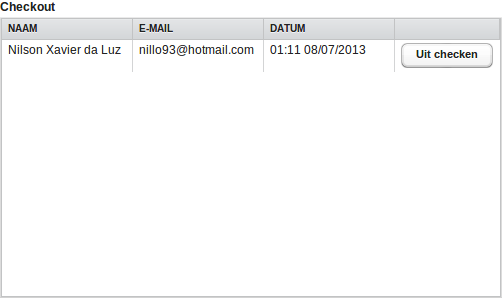
\includegraphics[width=0.65\textwidth]{Images/checkout-table.png}
	\caption{Pagina waar kan worden ingecheckt en uitgecheckt}
	\label{fig:checkout-table}
\end{figure}

\subsection{Checkout}

Wanneer de gebruiker klaar is en het lab wilt verlaten, wordt hij verzocht om eerste uit te checken. Dit gebeurt door zijn eigen informatie op te zoeken in de tabel en op de ``Uit checken'' knop te drukken. Er verschijnt dan een nieuwe venster om de benodigde informatie in te vullen over het project. Dit venster is weergegeven in Figuur \ref{fig:checkout-window}.

\begin{figure}[ht]
	\centering
	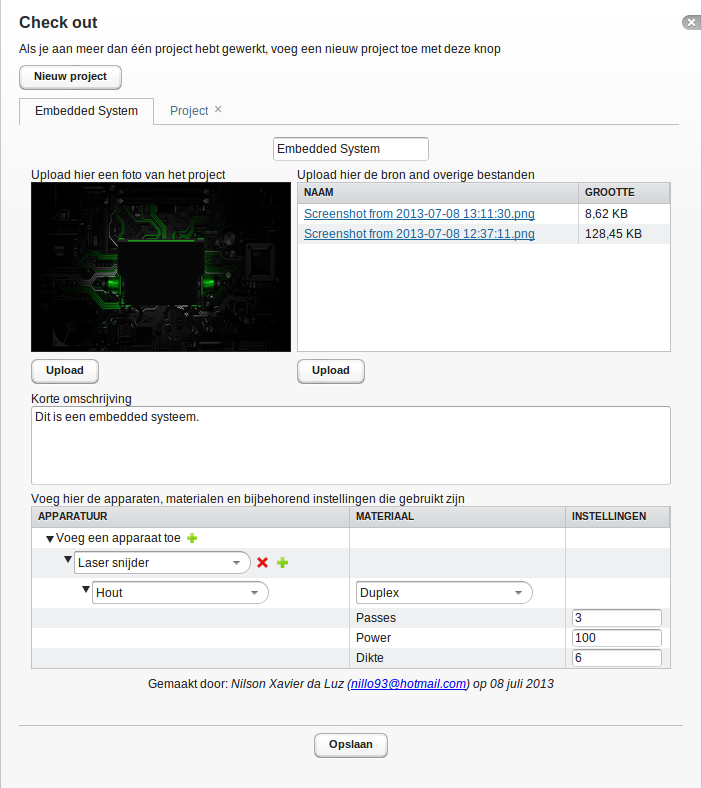
\includegraphics[width=0.65\textwidth]{Images/checkout-window.png}
	\caption{Venster waar kan worden uitgecheckt}
	\label{fig:checkout-window}
\end{figure}